\documentclass[aps,prl,reprint,amsmath,amssymb,nofootinbib,raggedbottom]{revtex4-2}
\usepackage[T1]{fontenc}
\usepackage{bm}
\usepackage{tikz}
\usetikzlibrary{arrows.meta}
\definecolor{mpoblue}{HTML}{5B9DBD}
\definecolor{mpored}{HTML}{D9666B}
\tikzset{
 tensor/.style={draw=black,fill=mpoblue,line width=.6pt,
   minimum width=.18cm,minimum height=.18cm,inner sep=0pt},
 wire/.style={draw=black,line width=.6pt},
 arrow/.style={-{Latex[length=1.5mm]},line width=.6pt}
}
\usepackage[colorlinks=true,citecolor=blue,linkcolor=blue,urlcolor=blue]{hyperref}
\hypersetup{pdftitle={A thermal-MPO derivation of the spin-1 gap bound}}
\newcommand{\Tr}{\operatorname{Tr}}
\newcommand{\Ps}{P_{\mathrm{s}}}
\newcommand{\Pt}{P_{\tau}}
\newcommand{\trv}{\operatorname{Tr}_{\mathrm v}}
\newenvironment{proofdiagram}{\par\smallskip\noindent\begin{minipage}{\columnwidth}\centering}{\end{minipage}\par\smallskip}
% A closed spacetime patch. Its opposite boundaries are identified.
% Arguments: lower-left x, lower-left y, number of columns, number of rows.
\newcommand{\netpatch}[4]{%
 \begin{scope}[shift={(#1,#2)}]
 \fill[mpoblue!10] (0,0) rectangle ({.4*#3},{.4*#4});
 \draw[black!35,densely dashed,line width=.35pt]
   (0,0) rectangle ({.4*#3},{.4*#4});
 \foreach \i in {1,...,#3}{
   \draw[wire] ({.4*\i-.2},0)--({.4*\i-.2},{.4*#4});}
 \foreach \j in {1,...,#4}{
   \draw[wire] (0,{.4*\j-.2})--({.4*#3},{.4*\j-.2});
   \foreach \i in {1,...,#3}{
     \node[tensor,minimum size=.10cm] at ({.4*\i-.2},{.4*\j-.2}) {};}}
 \end{scope}}

\begin{document}
\title{A thermal-MPO derivation of the spin-1 gap bound}
% Add author and affiliation information before circulation.
\date{October 7, 2026}
\begin{abstract}
Assuming two finite-size estimates from \emph{The periodic spin-one
Haldane gap}, we prove $\Delta_L>(\log20)/784$ for every even $L\ge2304$.
An exact thermal matrix product operator (MPO) relates the purities of
its spatial transfer operator and the Gibbs state. These purities control
the excited-state weight as the chain grows. Numerical certification of
the starting estimates is assumed.
\end{abstract}
\maketitle
\setlength{\abovedisplayskip}{5pt plus 2pt minus 1pt}
\setlength{\belowdisplayskip}{5pt plus 2pt minus 1pt}

We consider the antiferromagnetic spin-1 Heisenberg chain with periodic
boundary conditions $\bm S_{L+1}=\bm S_1$ and $J=k_B=1$:
\begin{equation}
 H_L=\sum_{j=1}^L\bm S_j\cdot\bm S_{j+1},\qquad
 Z_L(\beta)=\Tr e^{-\beta H_L}.
 \label{eq:model}
\end{equation}
All system sizes are even and at least four. Let
$E_0(L)\le E_1(L)\le\cdots$ include multiplicities and define the gap
$\Delta_L=E_1(L)-E_0(L)$. For the Gibbs weights
$w_m=e^{-\beta E_m(L)}/Z_L(\beta)$,
\begin{equation}
 \frac{w_1}{w_0}=e^{-\beta\Delta_L}\le e^{-c\beta}
 \quad\Longrightarrow\quad \Delta_L\ge c.
 \label{eq:target}
\end{equation}
To make $c$ independent of $L$, we first use a spatial transfer operator
to propagate a Gibbs-purity bound when $L$ and $\beta$ double. We then
extend the bound to intermediate lengths and apply Eq.~\eqref{eq:target}.
In the diagrams, horizontal legs are virtual indices, vertical legs are
physical indices, and connected legs are contracted \cite{tang,pirvu}.

\emph{Thermal MPO.---}
To obtain a real symmetric transfer operator, use the Cartesian spin
basis $s,s'\in\{x,y,z\}$. The matrices
$(S^\mu)_{ss'}=-i\epsilon_{\mu ss'}$ give real operators $G_\mu=iS^\mu$,
$\|G_\mu\|=1$, and $-H_L=\sum_{j,\mu}G_{\mu,j}G_{\mu,j+1}$.
Each bond event $(\tau,\mu)$ in the exponential expansion inserts
$G_\mu$ at both endpoints. Let $a,b$ record these events on the two bonds
adjacent to a site, with $0<\tau<\beta$. The local MPO tensor is
\begin{equation}
 W_\beta^{ss'}(a,b)=
 \left\langle s\left|\mathcal T_\tau
 \prod_{(\tau,\mu)\in a\cup b}G_\mu\right|s'\right\rangle.
 \label{eq:local}
\end{equation}
Here $\mathcal T_\tau$ places later times to the left. Summing event labels
and integrating ordered times defines a measure $\mu_\beta$ of mass
$e^{3\beta}$, with unit mass for the empty history. Contracting $L$ tensors
around the ring recovers the absolutely convergent exponential series.
This MPO is exact, with virtual space $L^2(\mu_\beta)$ and no bond
truncation; for Trotter-based constructions, see Ref.~\cite{pirvu}.

The transfer kernel $\mathbb T_\beta(a,b)=\sum_s W_\beta^{ss}(a,b)$
is real, symmetric, and bounded in absolute value by three.
It is therefore self-adjoint and Hilbert--Schmidt on $L^2(\mu_\beta)$.
Its eigenvalues $\lambda_i(\beta)$ give, for even $L$,
\begin{equation}
 Z_L(\beta)=\trv \mathbb T_\beta^L=\sum_i|\lambda_i(\beta)|^L.
 \label{eq:moment}
\end{equation}

\begin{proofdiagram}
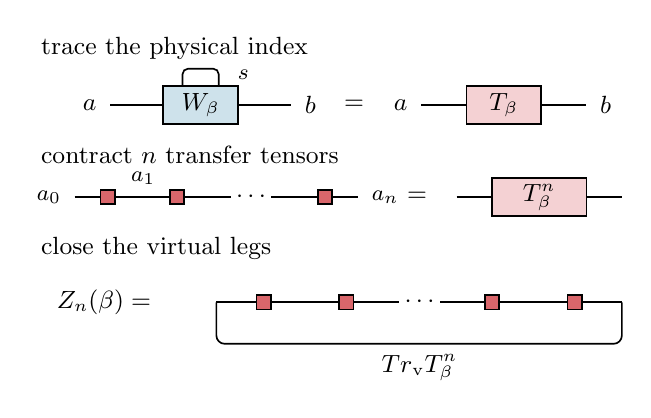
\begin{tikzpicture}[x=1cm,y=.85cm,font=\small]
 % The two physical legs are drawn upward and joined to take their trace.
 \node[anchor=west] at (.15,5.35) {trace the physical index};
 \draw[wire] (1.15,4.50)--(3.45,4.50);
 \draw[wire,rounded corners=2pt]
   (2.07,4.70)--(2.07,5.04)--(2.53,5.04)--(2.53,4.70);
 \node[tensor,fill=mpoblue!30,minimum width=.95cm,minimum height=.48cm]
   at (2.30,4.50) {$W_\beta$};
 \node[font=\footnotesize,anchor=west] at (2.65,4.95) {$s$};
 \node[anchor=east] at (1.10,4.50) {$a$};
 \node[anchor=west] at (3.50,4.50) {$b$};
 \node at (4.25,4.50) {$=$};
 \draw[wire] (5.10,4.50)--(7.20,4.50);
 \node[tensor,fill=mpored!30,minimum width=.95cm,minimum height=.48cm]
   at (6.15,4.50) {$\mathbb T_\beta$};
 \node[anchor=east] at (5.05,4.50) {$a$};
 \node[anchor=west] at (7.25,4.50) {$b$};
 % Open virtual legs give an operator on the virtual space.
 \node[anchor=west] at (.15,3.75) {contract $n$ transfer tensors};
 \draw[wire] (.70,3.12)--(4.30,3.12);
 \foreach \x in {1.12,2.00,3.88}{
   \node[tensor,fill=mpored] at (\x,3.12) {};}
 \node[fill=white,inner sep=2pt] at (2.94,3.12) {$\cdots$};
 \node[font=\footnotesize] at (1.57,3.40) {$a_1$};
 \node[font=\footnotesize,anchor=east] at (.65,3.12) {$a_0$};
 \node[font=\footnotesize,anchor=west] at (4.35,3.12) {$a_n$};
 \node at (5.05,3.12) {$=$};
 \draw[wire] (5.55,3.12)--(7.65,3.12);
 \node[tensor,fill=mpored!30,minimum width=1.20cm,minimum height=.48cm]
   at (6.60,3.12) {$\mathbb T_\beta^n$};
 % Closing the two remaining virtual legs gives the partition function.
 \node[anchor=west] at (.15,2.35) {close the virtual legs};
 \node[anchor=west] at (.35,1.55) {$Z_n(\beta)=$};
 \draw[wire] (2.50,1.55)--(7.65,1.55);
 \draw[wire,rounded corners=3pt]
   (2.50,1.55)--(2.50,.93)--(7.65,.93)--(7.65,1.55);
 \foreach \x in {3.10,4.15,6.00,7.05}{
   \node[tensor,fill=mpored] at (\x,1.55) {};}
 \node[fill=white,inner sep=2pt] at (5.08,1.55) {$\cdots$};
 \node at (5.08,.57) {$\trv\mathbb T_\beta^n$};
\end{tikzpicture}
\end{proofdiagram}
The loop on $W_\beta$ sums $s=s'$. The red chain has open virtual legs;
closing them takes the virtual trace $\trv$ over $a_0=a_n$.


\emph{Purity and excited-state weight.---}
We want one Gibbs weight to be close to one. For a positive trace-one
operator with eigenvalues $p_i$ and $p_{\max}=\max_i p_i$, the purity obeys
\begin{equation}
 P=\sum_i p_i^2\le p_{\max}\sum_i p_i=p_{\max}.
 \label{eq:weight}
\end{equation}
Thus $1-p_{\max}\le1-P$. For the Gibbs state, $P>1/2$ implies a unique
ground state, with excited-state population $1-w_0\le1-P$.

To propagate this bound, normalize both the transfer and Gibbs operators:
\begin{equation}
 \sigma_n(\beta)=\frac{\mathbb T_\beta^n}{Z_n(\beta)},\qquad
 \rho_n(\beta)=\frac{e^{-\beta H_n}}{Z_n(\beta)}.
 \label{eq:states}
\end{equation}
Here $\sigma_n$ is the open red chain divided by its closed-loop value.
Both operators are positive with unit trace; denote their eigenvalues by
$p_i$ and $w_m$, respectively. Their purities are
$\Ps(n,\beta)=\trv\sigma_n(\beta)^2$ and
$\Pt(n,\beta)=\Tr\rho_n(\beta)^2$.
Squaring $\sigma_n$ doubles the length; squaring $\rho_n$ doubles the
inverse temperature:
\begin{proofdiagram}
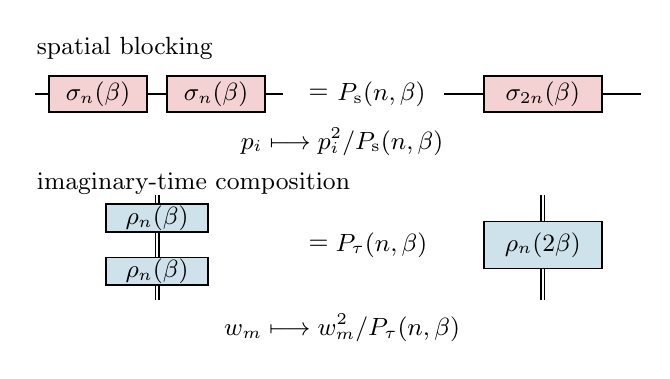
\begin{tikzpicture}[x=1cm,y=.90cm,font=\small]
 \node[anchor=west] at (0,2.00) {spatial blocking};
 \draw[wire] (.1,1.35)--(3.25,1.35);
 \node[tensor,fill=mpored!30,minimum width=1.25cm,minimum height=.45cm] at (.90,1.35) {$\sigma_n(\beta)$};
 \node[tensor,fill=mpored!30,minimum width=1.25cm,minimum height=.45cm] at (2.40,1.35) {$\sigma_n(\beta)$};
 \node at (3.70,1.35) {$=$};
 \node at (4.50,1.35) {$\Ps(n,\beta)$};
 \draw[wire] (5.30,1.35)--(7.80,1.35);
 \node[tensor,fill=mpored!30,minimum width=1.5cm,minimum height=.45cm] at (6.55,1.35) {$\sigma_{2n}(\beta)$};
 \node at (4,.68) {$p_i\longmapsto p_i^2/\Ps(n,\beta)$};
 \node[anchor=west] at (0,.08) {imaginary-time composition};
 \draw[wire,double distance=.6pt] (1.65,-.08)--(1.65,-1.55);
 \node[tensor,fill=mpoblue!30,minimum width=1.3cm,minimum height=.35cm] at (1.65,-.40) {$\rho_n(\beta)$};
 \node[tensor,fill=mpoblue!30,minimum width=1.3cm,minimum height=.35cm] at (1.65,-1.15) {$\rho_n(\beta)$};
 \node at (3.70,-.78) {$=$};
 \node at (4.50,-.78) {$\Pt(n,\beta)$};
 \draw[wire,double distance=.6pt] (6.55,-.08)--(6.55,-1.55);
 \node[tensor,fill=mpoblue!30,minimum width=1.5cm,minimum height=.6cm] at (6.55,-.78) {$\rho_n(2\beta)$};
 \node at (4,-1.95) {$w_m\longmapsto w_m^2/\Pt(n,\beta)$};
\end{tikzpicture}
\end{proofdiagram}
A double leg denotes the $n$-site physical space. Taking traces gives
\begin{equation}
 \Ps(n,\beta)=\frac{Z_{2n}(\beta)}{Z_n(\beta)^2},\qquad
 \Pt(n,\beta)=\frac{Z_n(2\beta)}{Z_n(\beta)^2}.
 \label{eq:purities}
\end{equation}
Both operations replace normalized eigenvalues $p_i$ by $p_i^2/P$.
To bound the new purity $P'$, use $1-P=2\sum_{i<k}p_ip_k$:

\begin{equation}
 1-P'=\frac{2\sum_{i<k}p_i^2p_k^2}{P^2}
 \le\frac{(1-P)^2}{2P^2}=:f(1-P).
 \label{eq:square}
\end{equation}
Dropping cross terms from $(\sum_{i<k}p_ip_k)^2$ gives the inequality.
Here $f$ increases on $[0,1)$, with $f(x)\sim x^2/2$ for small $x$.

\emph{Joining copies in space and time.---}
Squaring controls $\Ps$ when $n$ doubles and $\Pt$ when $\beta$ doubles.
To double both variables, we also need to relate $\Ps$ and $\Pt$.
Rejoin the trace loops of four copies of $Z_n(\beta)$ in either order.
Each rectangle is periodic; its width and height denote length and
inverse temperature. Tensors are schematic; arrows give ratios of
new to old contraction values.
\begin{proofdiagram}
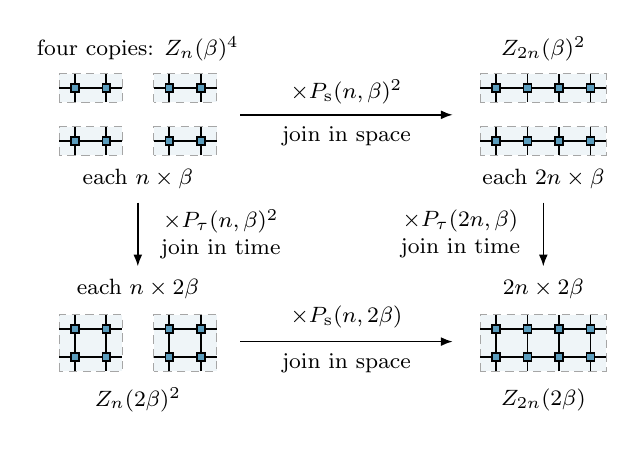
\begin{tikzpicture}[x=1cm,y=.90cm,font=\footnotesize]
 \netpatch{.35}{3.75}{2}{1}
 \netpatch{1.55}{3.75}{2}{1}
 \netpatch{.35}{4.50}{2}{1}
 \netpatch{1.55}{4.50}{2}{1}
 \node at (1.35,5.25) {four copies: $Z_n(\beta)^4$};
 \node at (1.35,3.42) {each $n\times\beta$};
 \netpatch{5.70}{3.75}{4}{1}
 \netpatch{5.70}{4.50}{4}{1}
 \node at (6.50,5.25) {$Z_{2n}(\beta)^2$};
 \node at (6.50,3.42) {each $2n\times\beta$};
 \draw[arrow] (2.65,4.32)--(5.35,4.32);
 \node at (4,4.64) {$\times \Ps(n,\beta)^2$};
 \node at (4,4.02) {join in space};
 \netpatch{.35}{.70}{2}{2}
 \netpatch{1.55}{.70}{2}{2}
 \node at (1.35,.30) {$Z_n(2\beta)^2$};
 \node at (1.35,1.86) {each $n\times2\beta$};
 \netpatch{5.70}{.70}{4}{2}
 \node at (6.50,.30) {$Z_{2n}(2\beta)$};
 \node at (6.50,1.86) {$2n\times2\beta$};
 \draw[arrow] (2.65,1.12)--(5.35,1.12);
 \node at (4,1.47) {$\times \Ps(n,2\beta)$};
 \node at (4,.81) {join in space};
 \draw[arrow] (1.35,3.08)--(1.35,2.18);
 \node[align=center,anchor=west] at (1.52,2.64)
   {$\times \Pt(n,\beta)^2$\\join in time};
 \draw[arrow] (6.50,3.08)--(6.50,2.18);
 \node[align=center,anchor=east] at (6.33,2.64)
   {$\times \Pt(2n,\beta)$\\join in time};
\end{tikzpicture}
\end{proofdiagram}
Both orders give $Z_{2n}(2\beta)$. Equating their ratios, then using
the same identity at $2n$, gives
\begin{align}
 \Ps(n,2\beta)&=\frac{\Ps(n,\beta)^2\Pt(2n,\beta)}{\Pt(n,\beta)^2},
 \label{eq:couple1}\\
 \Pt(4n,\beta)&=\frac{\Pt(2n,\beta)^2\Ps(2n,2\beta)}{\Ps(2n,\beta)^2}.
 \label{eq:couple2}
\end{align}
\emph{Doubling estimate.---}
We now prove that, for $0\le\varepsilon\le1/100$,
\begin{equation}
 \begin{gathered}
 \Ps(n,\beta),\ \Pt(2n,\beta)\ge1-\varepsilon\\
 \Longrightarrow\quad
 \Ps(2n,2\beta),\ \Pt(4n,2\beta)\ge1-5\varepsilon^2.
 \end{gathered}
 \label{eq:update}
\end{equation}
The lengths $n$ and $2n$ let the identities above reproduce this pair
of purities at the next scale.

First bound the new transfer purity. Since $\Pt(n,\beta)\le1$,
Eq.~\eqref{eq:couple1} gives $\Ps(n,2\beta)\ge(1-\varepsilon)^3$.
Spatial blocking and Eq.~\eqref{eq:square} therefore give
$\Ps(2n,2\beta)\ge1-\delta$, where
\begin{equation}
 \delta=f\bigl(1-(1-\varepsilon)^3\bigr)
 =\tfrac12\bigl[(1-\varepsilon)^{-3}-1\bigr]^2
 \le5\varepsilon^2\le\varepsilon.
 \label{eq:delta}
\end{equation}
Here we used $1-(1-\varepsilon)^3\le3\varepsilon$ and
$9/[2(1-3\varepsilon)^2]\le5$.

Now bound the new Gibbs purity. Inserting the transfer bound into
Eq.~\eqref{eq:couple2}, with $\delta\le\varepsilon$, gives
$\Pt(4n,\beta)\ge(1-\varepsilon)^3$.
Squaring the Gibbs operator then gives $\Pt(4n,2\beta)\ge1-\delta$ by
Eq.~\eqref{eq:square}. This proves both bounds in Eq.~\eqref{eq:update}.

\par\smallskip\noindent\begin{minipage}{\columnwidth}
\emph{Finite input and iteration.---}
We start the iteration from Proposition~5.5 of Ref.~\cite{source}:
\begin{equation}
 \Ps(2304,784),\ \Pt(4608,784)\ge0.99.
 \label{eq:input}
\end{equation}
\end{minipage}\par\smallskip
The energy shift used there cancels from the purity ratios.
After $j\ge0$ doublings, set
\begin{equation}
 n_j=2304\,2^j,\qquad \beta_j=784\,2^j,\qquad
 \varepsilon_j=\frac{20^{-2^j}}5.
 \label{eq:scales}
\end{equation}
Since $\varepsilon_0=1/100$ and $\varepsilon_{j+1}=5\varepsilon_j^2$,
Eq.~\eqref{eq:update} gives
$\Ps(n_j,\beta_j),\Pt(2n_j,\beta_j)\ge1-\varepsilon_j$.
The error $\varepsilon_j=\frac15\exp[-\beta_j(\log20)/784]$ decays
exponentially in inverse temperature, as needed in Eq.~\eqref{eq:target}.

These estimates hold at the doubled lengths. To cover every even
$L\ge2304$, choose $j$ with $n_j\le L\le2n_j$.
Monotonicity of the $\ell^p$ norms in Eq.~\eqref{eq:moment} gives
\begin{align}
 Z_L(\beta_j)&\le Z_{n_j}(\beta_j)^{L/n_j},\notag\\
 Z_L(2\beta_j)&\ge Z_{2n_j}(2\beta_j)^{L/(2n_j)}.
 \label{eq:moments}
\end{align}
Substitution into the Gibbs-purity ratio gives
\begin{align}
 \Pt(L,\beta_j)
 &\ge\bigl[\Pt(2n_j,\beta_j)\Ps(n_j,\beta_j)^2\bigr]^{L/(2n_j)}\notag\\
 &\ge(1-\varepsilon_j)^3\ge1-3\varepsilon_j>\tfrac12.
 \label{eq:interpolate}
\end{align}
Here $L/(2n_j)\le1$, and both purities in brackets are at least
$1-\varepsilon_j$.

\emph{Recovering the gap.---}
We can now apply Eq.~\eqref{eq:target}. Order the eigenvalues
of $\rho_L(\beta_j)$ as $w_0\ge w_1\ge\cdots$.
By Eqs.~\eqref{eq:weight} and \eqref{eq:interpolate},
$w_0\ge1-3\varepsilon_j>1/2$. Two ground states would have equal
largest weights, so the ground state is unique. The remaining weight
bounds $w_1$, and hence
\begin{equation}
 e^{-\beta_j\Delta_L}=\frac{w_1}{w_0}
 \le\frac{1-w_0}{w_0}
 \le\frac{3\varepsilon_j}{1-3\varepsilon_j}
 <20^{-2^j}.
 \label{eq:gapratio}
\end{equation}
The last inequality uses
$3\varepsilon_j/(1-3\varepsilon_j)\le(60/97)20^{-2^j}$.
Taking logarithms and dividing by $\beta_j=784\,2^j$ gives, for every
even $L\ge2304$,
\begin{equation}
 \boxed{\Delta_L>\frac{\log20}{784}\simeq0.003821.}
 \label{eq:gap}
\end{equation}
Hence $\liminf_{L\to\infty,\;L\,\mathrm{even}}\Delta_L
\ge(\log20)/784>0$, conditional on Eq.~\eqref{eq:input}.

\begin{thebibliography}{3}
\bibitem{source}
OpenAI, \emph{The periodic spin-one Haldane gap}, manuscript dated
September 24, 2026, Proposition 5.5 and Appendices A--C.
\bibitem{tang}
W. Tang, H.-H. Tu, and L. Wang,
\href{https://doi.org/10.1103/PhysRevLett.125.170604}
{Continuous matrix product operator approach to finite temperature quantum states},
Phys. Rev. Lett. \textbf{125}, 170604 (2020).
\bibitem{pirvu}
B. Pirvu, V. Murg, J. I. Cirac, and F. Verstraete,
\href{https://doi.org/10.1088/1367-2630/12/2/025012}
{Matrix product operator representations},
New J. Phys. \textbf{12}, 025012 (2010).
\end{thebibliography}
\end{document}
